% Skipping a bunch of chapters
\chapter{Exascale Cyberinfrastructure}

\section{Rucio}

\section{SENSE}

\begin{figure}[htb]
  \centering
  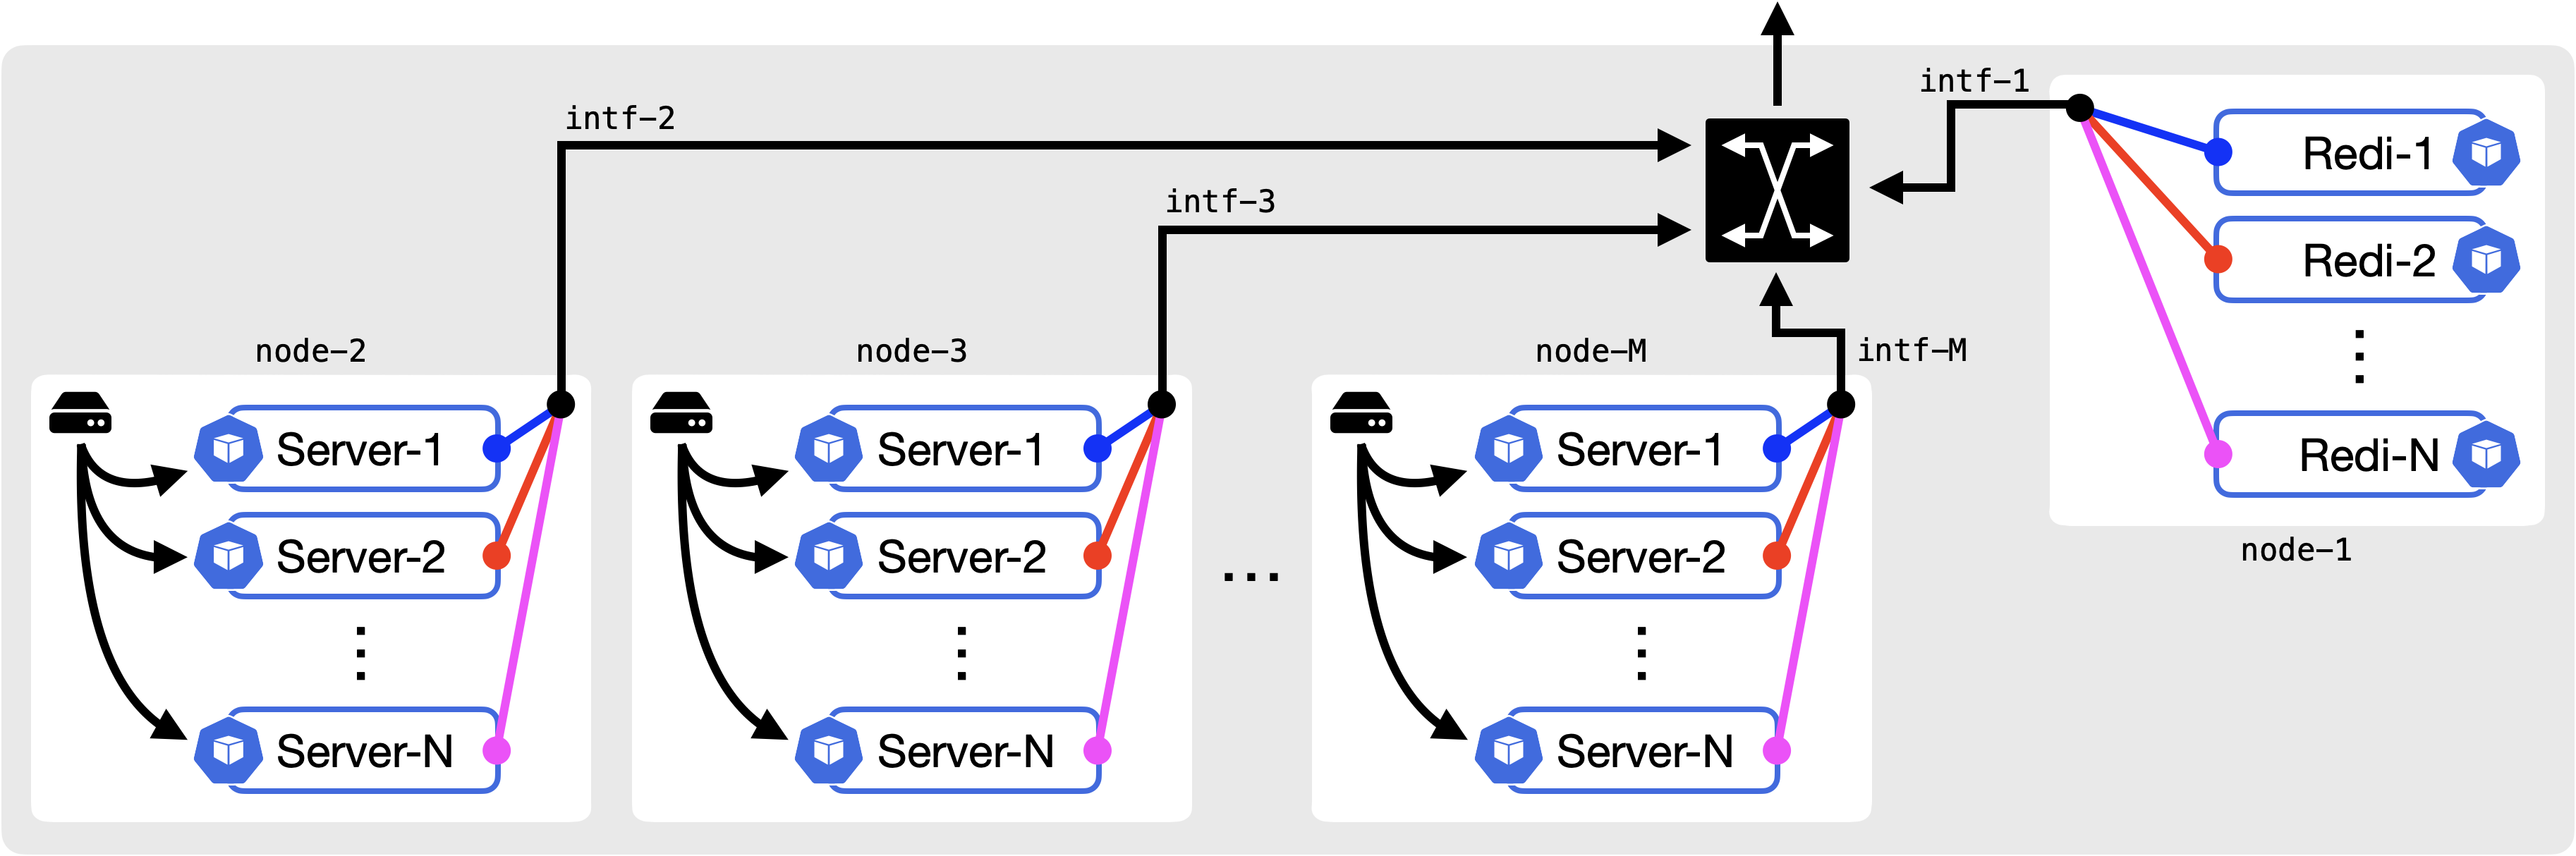
\includegraphics[width=.9\textwidth]{fig/cyber/rucio-sense_site.png}
  \caption{Lorem ipsum}
  \label{fig:rucio_sense_site}
\end{figure}

\section{Rucio-SENSE interoperation model}
% The central goal of this work is to produce a Rucio-SENSE interoperation model that enables Rucio operators to prioritize certain transfers, then see those priorities reflected in the allocation of network resources.
% Moreover, this should have a minimal impact on the current implementation and operation of Rucio.
% To this end, a Data Movement Manager (DMM) is introduced to perform the crucial task of translating Rucio requests into SENSE provisions and returning the
% results, keeping a bulk of the functionality required for the incorporation of SENSE capabilities separate from the Rucio codebase.
% Thus, DMM serves as a keystone for the Rucio-SENSE interoperation model explored in this initial work (Fig. \ref{fig:rucio_sense_basic}):
% \begin{enumerate}
%     \item A Rucio operator initializes a rule with some priority which requests one or more dataset transfers, where each transfer may involve a different pair (source and destination) of sites
%     \item Rucio sends the following data to DMM for each transfer:
%     \begin{itemize}
%         \item Total transfer size
%         \item Source site
%         \item Destination site
%         \item Priority
%     \end{itemize}
%     \item DMM processes the data from Rucio:
%     \begin{enumerate}
%         \item If the transfer has no priority, immediately place it on best effort service (skip steps below)
%         \item Reserve an IPv6 address at the source and destination site
%         \item Compute the bandwidth provision (i.e. promise) appropriate for the transfer priority
%     \end{enumerate}
%     \item DMM requests a new promise from SENSE that implements the provisioning from (3c), reprovisioning existing promises where appropriate
%     \item DMM sends the IPv6 addresses it reserved to Rucio
%     \item Rucio injects the IPv6 addresses into the FTS request
%     \item SENSE takes one of the following actions:
%     \begin{enumerate}
%         \item Begin the construction of a new guaranteed-bandwidth link
%         \item Do nothing; the transfer will be provided best effort service
%     \end{enumerate}
%     \item SENSE sends identifying metadata for the link back to DMM
% \end{enumerate}
% Several of these steps offer the opportunity for further optimization.
% In particular, it is clear that a future implementation may see the integration of DMM into Rucio such that the operations in steps (2) through (5) can be implemented to better handle a large number of transfers.
% Before then, however, DMM provides an isolated testbed in which the fundamental design of the interoperation model can be prototyped.
% Step (3c) is of particular interest, because it implements the bandwidth provisioning--the central deliverable of this work.
% The provisioning decision could be designed, for example, to allow Rucio operators to schedule transfers: e.g. \textit{move Dataset A to Site B in one week}.
% Alternatively, the decision could pack the maximum available bandwidth between two sites as a function of each transfer's priority.
% In any case, this interoperation model provides a flexible testbed for evaluating these ideas and producing concrete metrics on their scalability, practicality, and efficiency.

\begin{figure}[htb]
  \centering
  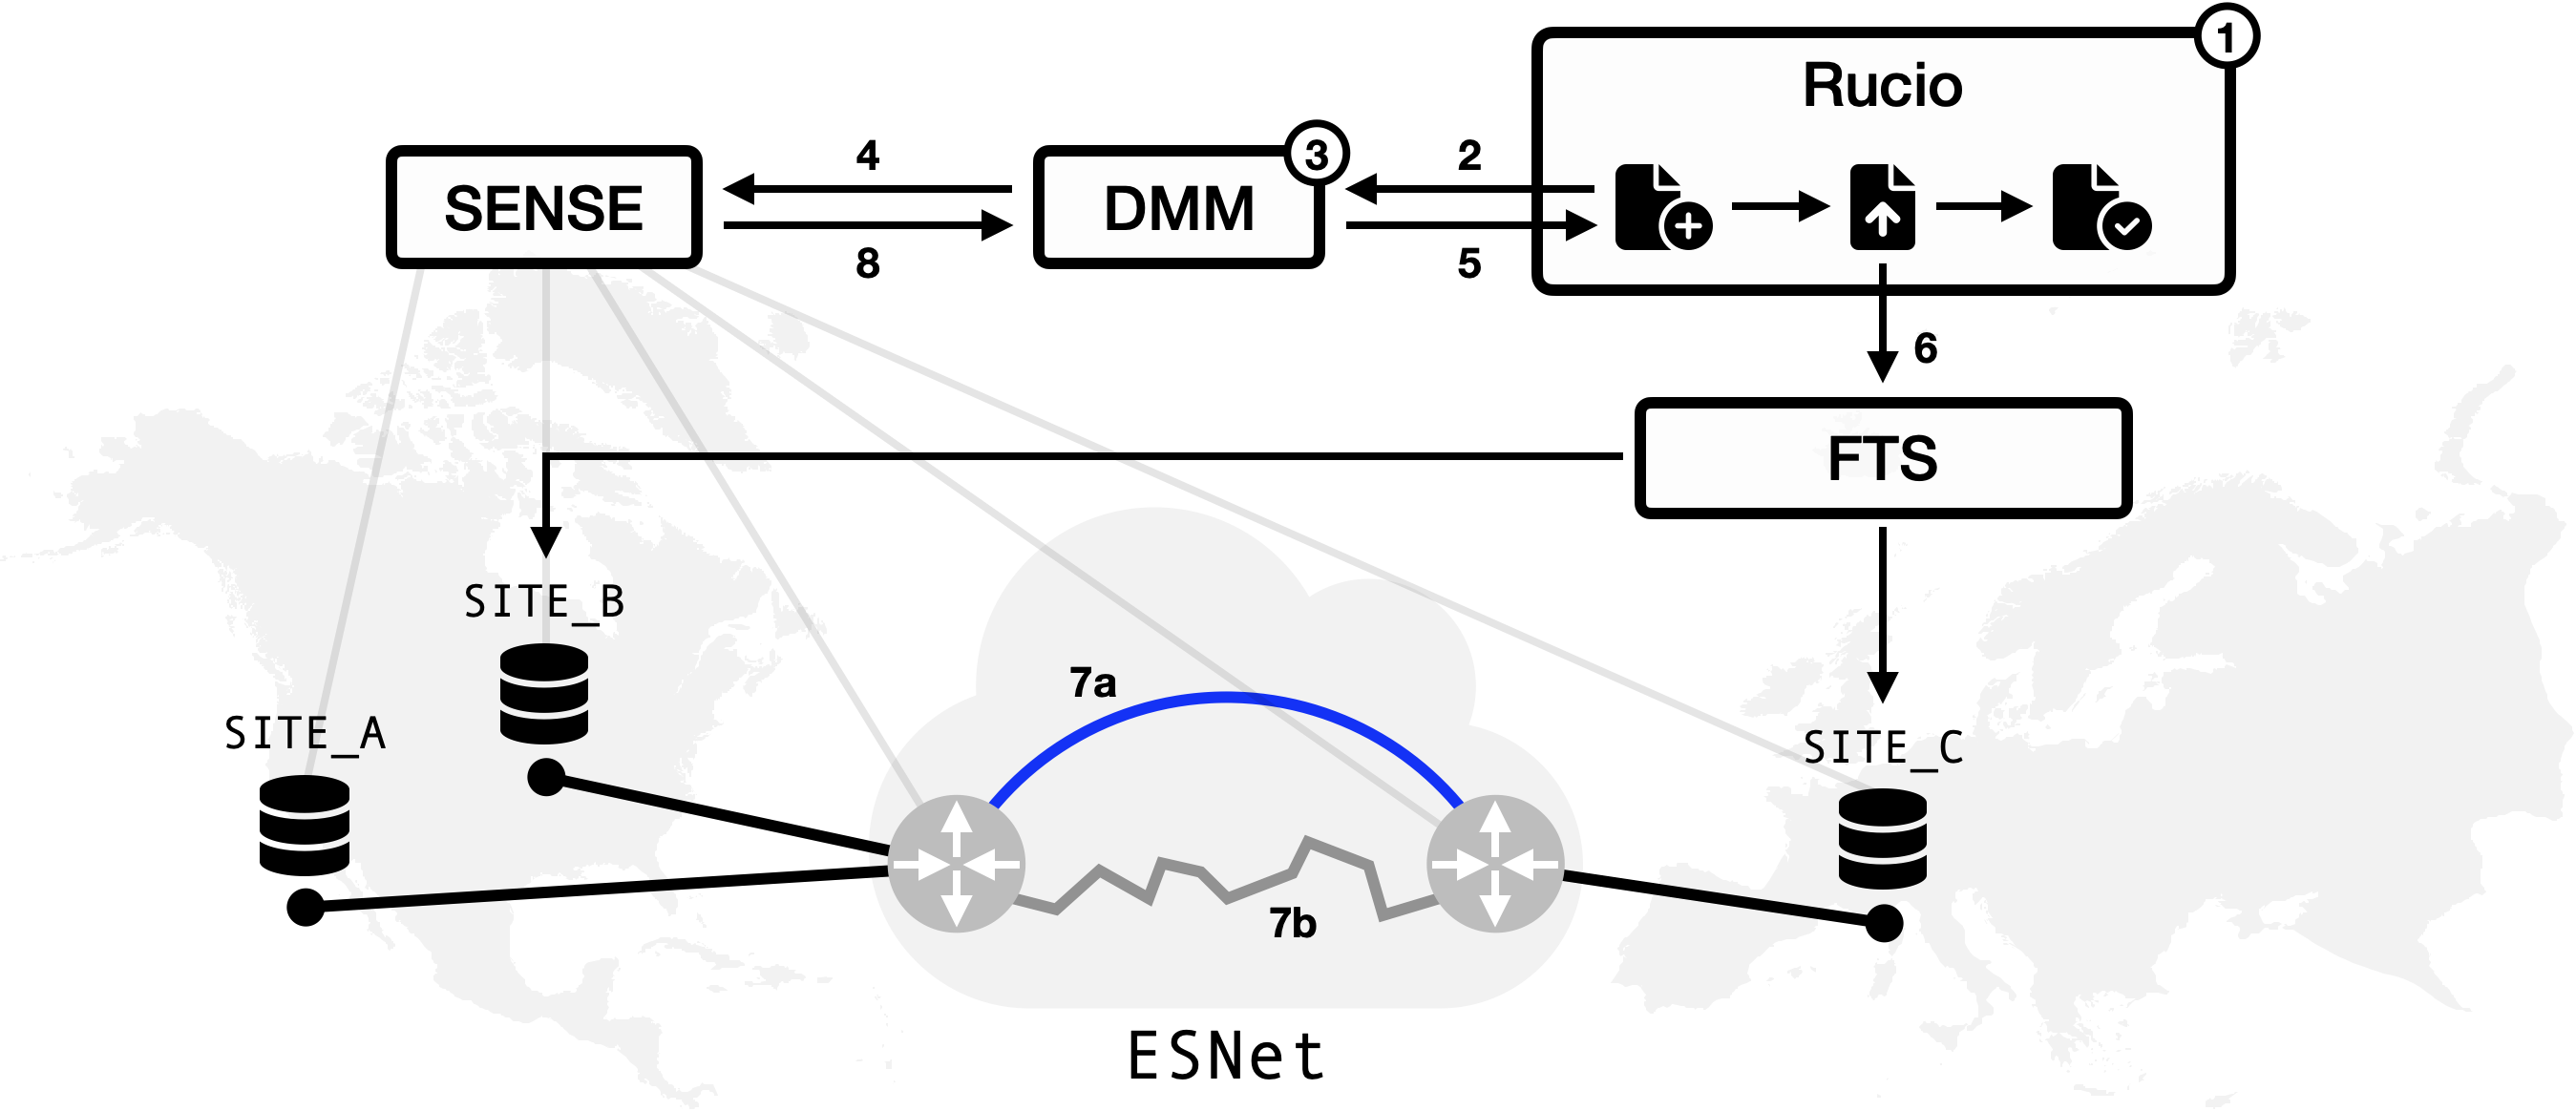
\includegraphics[width=.9\textwidth]{fig/cyber/rucio-sense_basic.png}
  \caption{
    Simplified diagram of the Rucio-SENSE interoperation workflow, with numbered steps: 
    (1) a rule is initialized; 
    (2) Rucio sends transfer description to DMM; 
    (3) DMM translates Rucio request into SENSE provision; 
    (4) DMM sends provision request to SENSE; 
    (5) DMM sends a source IPv6 and destination IPv6 to Rucio;
    (6) Rucio injects IPv6s from previous step into the FTS request;
    (7) Either (a) SENSE builds dedicated service or (b) default to best effort service; 
    (8) SENSE sends service metadata to DMM.
  }
  \label{fig:rucio_sense_basic}
\end{figure}

\section{Demonstration}

\begin{figure}[htb]
  \centering
  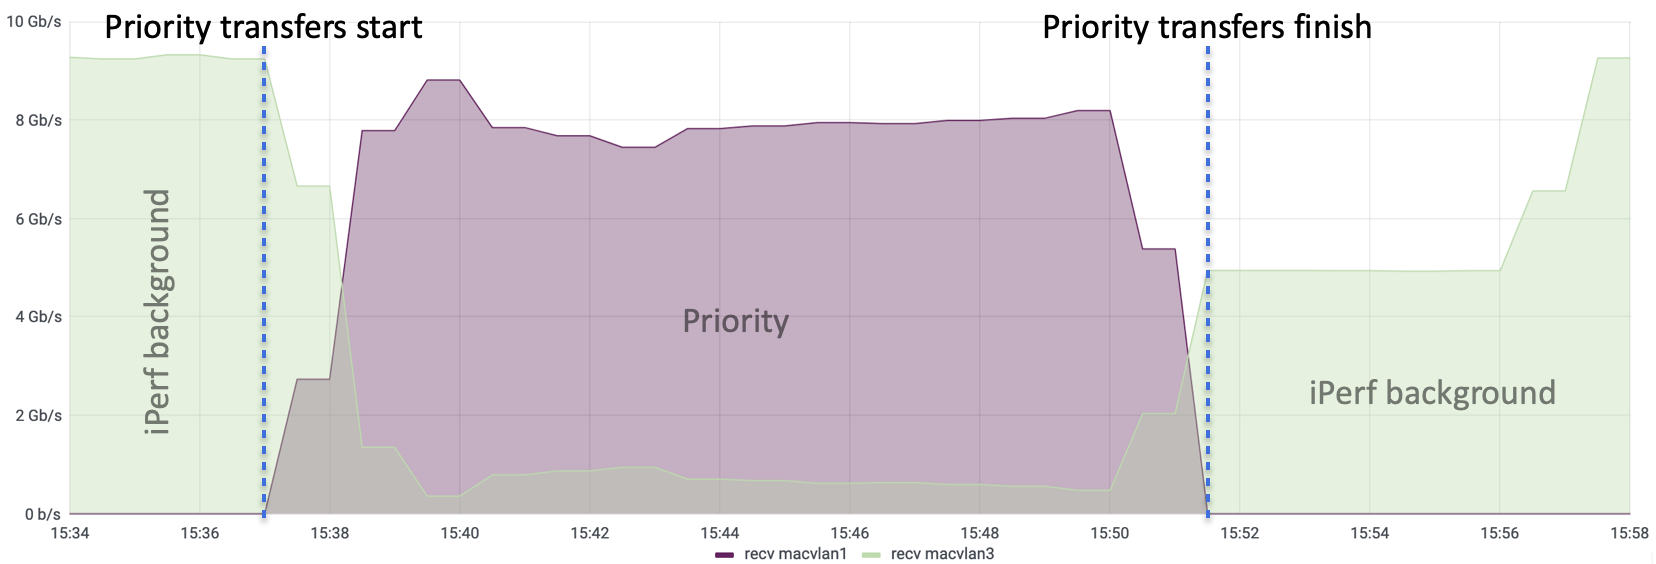
\includegraphics[width=.9\textwidth]{fig/cyber/rucio-sense_demo.png}
  \caption{Lorem ipsum}
  \label{fig:rucio_sense_demo}
\end{figure}
